\chapter{From ZDRa to General Proof Sketch}
\label{ch:skeletons}

The skeletons described in this chapter are automatically generated if the
specification passes the \gls{zdra} check. Section \ref{sec:buildinggraphs}
outlines how the dependency and goto graphs are generated from the \gls{zdra}
annotations. Then section \ref{sec:zdra2gen} describes how \gls{zmath} builds
the \gls{gps} from the graphs. 

\section{Building the Dependency and GoTo graphs}
\label{sec:buildinggraphs}

In this section we outline how the dependency graph is created from the
\gls{zdra} annotations. We see that each relation becomes an `\emph{edge}' in
the graph and each instance becomes a `\emph{node}' in the graph. The goto graph
is then built from the dependency graph with the same nodes but some edges being
reversed.

\subsection{How \gls{zmath} builds the dependency graph from the \gls{zdra} annotations}

We use the definitions from \cite{zengfirstyear} to describe `\emph{nodes}'
`\emph{relational edges}' to describe the dependency graph as a set.

\begin{defin}[Nodes] We can say a node of the graph (or vertex) $\mathbb{V}$, is
a pair.
\begin{center}
(id, ins)
\end{center}
of a unique identifier id, and instance name ins. 
\end{defin} 

\begin{defin}[Relational Edges] We can say a relation edge $\mathbb{E}$, is a
triple
\begin{center}
($n_{1}$, rel, $n_{2}$)
\end{center}
of a relation from node $v_{1}$ to $v_{2}$ with relation name rel.
\end{defin} 

We can now show the how annotations are represented and processed for the
dependency graph.

\begin{defin}[Dep graph set] A dependency graph $\mathbb{D}$, is a set of
relational edges and a set of nodes.\\
$\mathbb{D} = \mathbb{E} \cup \mathbb{V}$
\end{defin} 

Using the definitions from \cite{zengfirstyear}, we can group the nodes and
edges together to describe the \gls{zdra} annotations.

\begin{table}[H]
\begin{center}
\begin{tabular}{ |p{0.8cm} | l | l | }
\hline
$\mathbf{N^{o}}$ & \textbf{Annotations} &  \\ 
\hline
dra1) & 
\raisebox{-\totalheight}{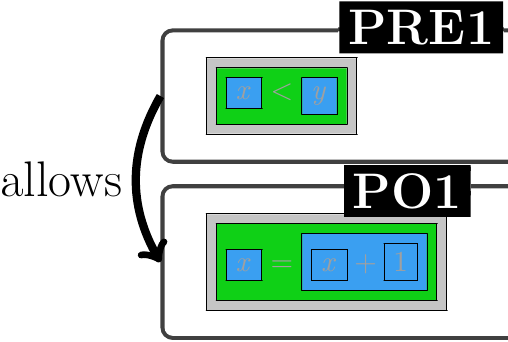
\includegraphics[scale=0.2]{Figures/Formalising/dra1.png}}
      &  
\raisebox{-\totalheight}{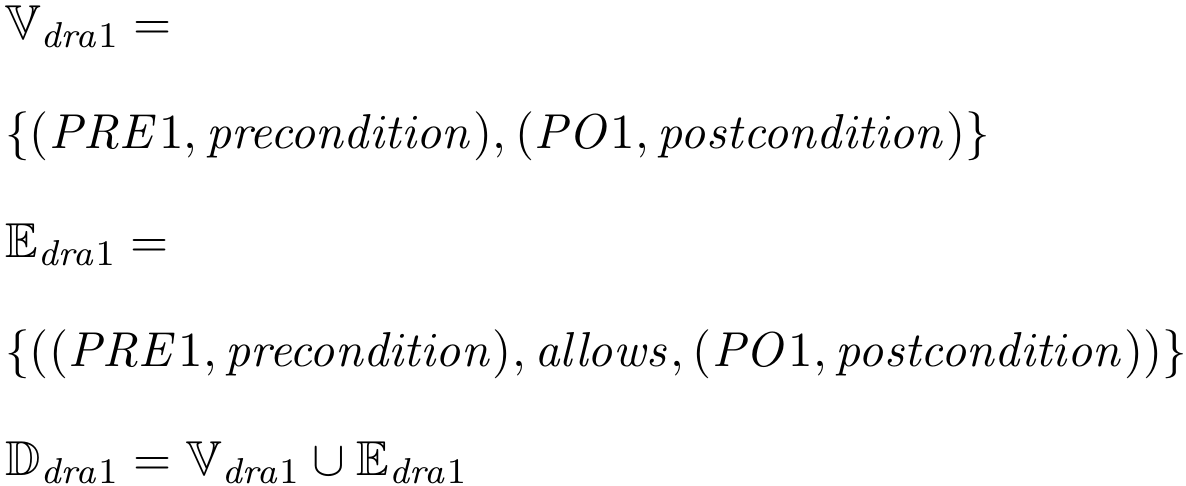
\includegraphics[scale=0.2]{Figures/Formalising/dra1txt.png}}
\\ \hline
dra2) & 
\raisebox{-\totalheight}{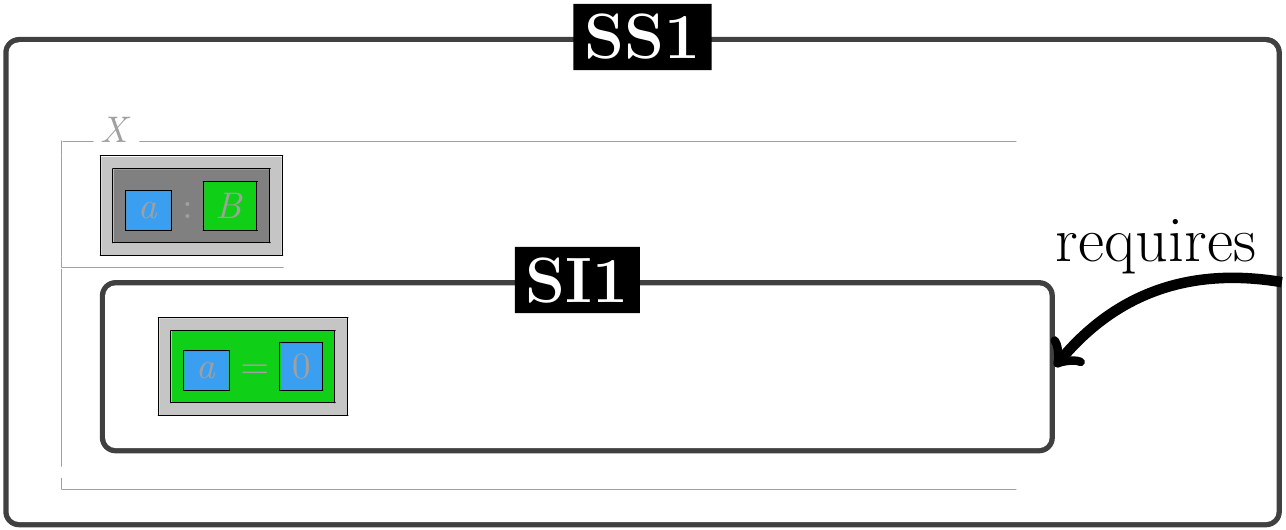
\includegraphics[scale=0.08]{Figures/Formalising/dra2.png}}
      &  
\raisebox{-\totalheight}{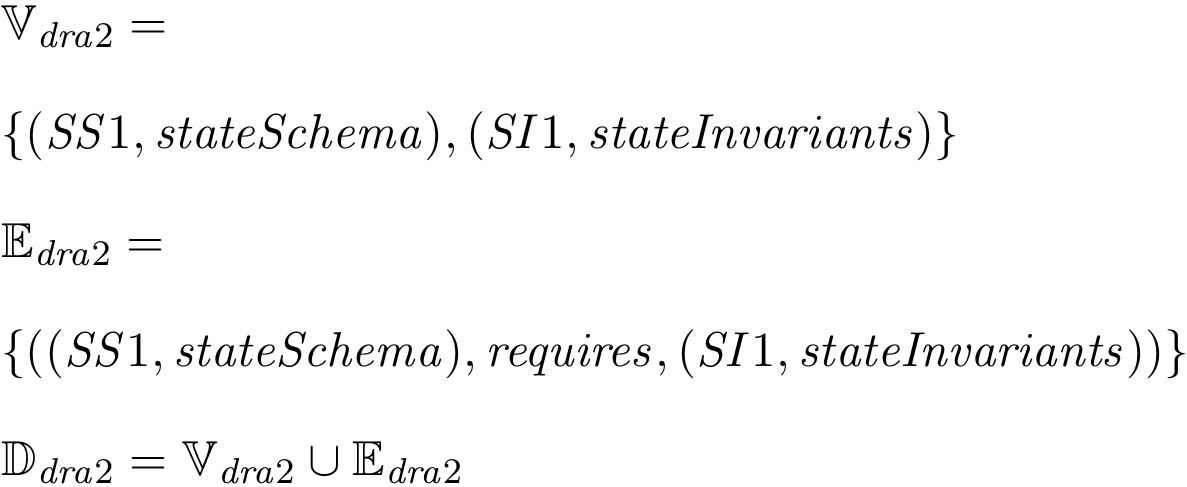
\includegraphics[scale=0.2]{Figures/Formalising/dra2txt.png}}
\\ \hline
dra3) & 
\raisebox{-\totalheight}{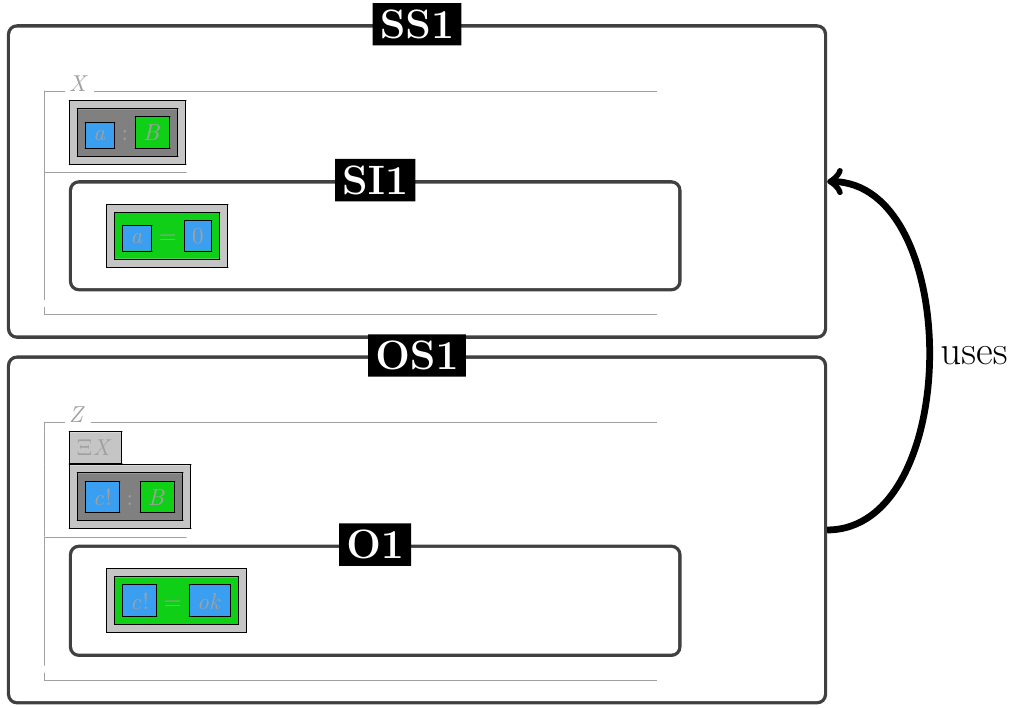
\includegraphics[scale=0.1]{Figures/Formalising/dra3.png}}
      &  
\raisebox{-\totalheight}{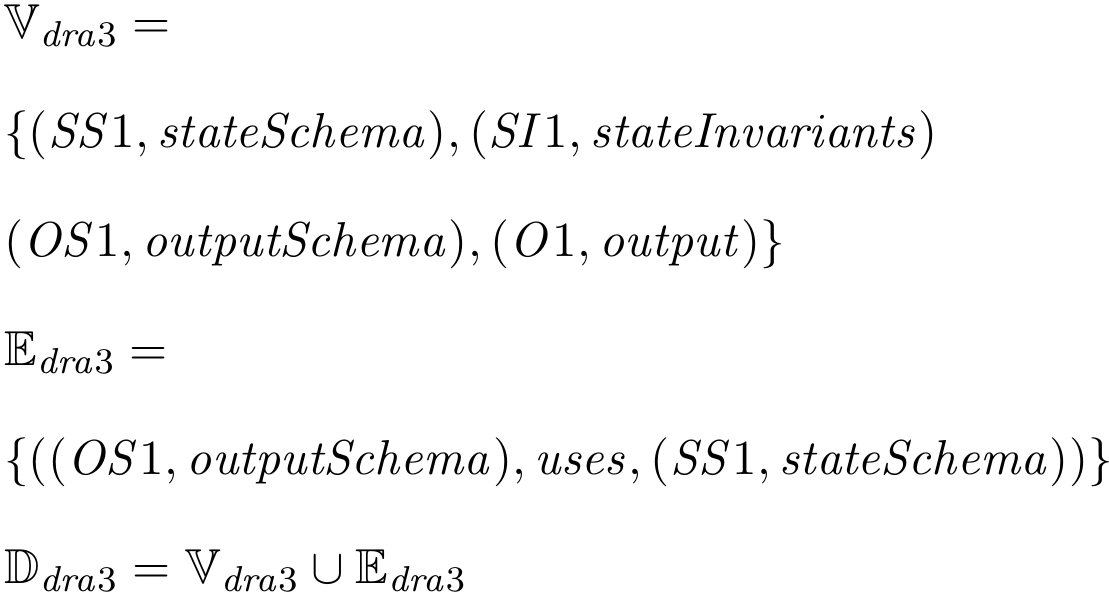
\includegraphics[scale=0.2]{Figures/Formalising/dra3txt.png}}
\\ \hline
dra4) & 
\raisebox{-\totalheight}{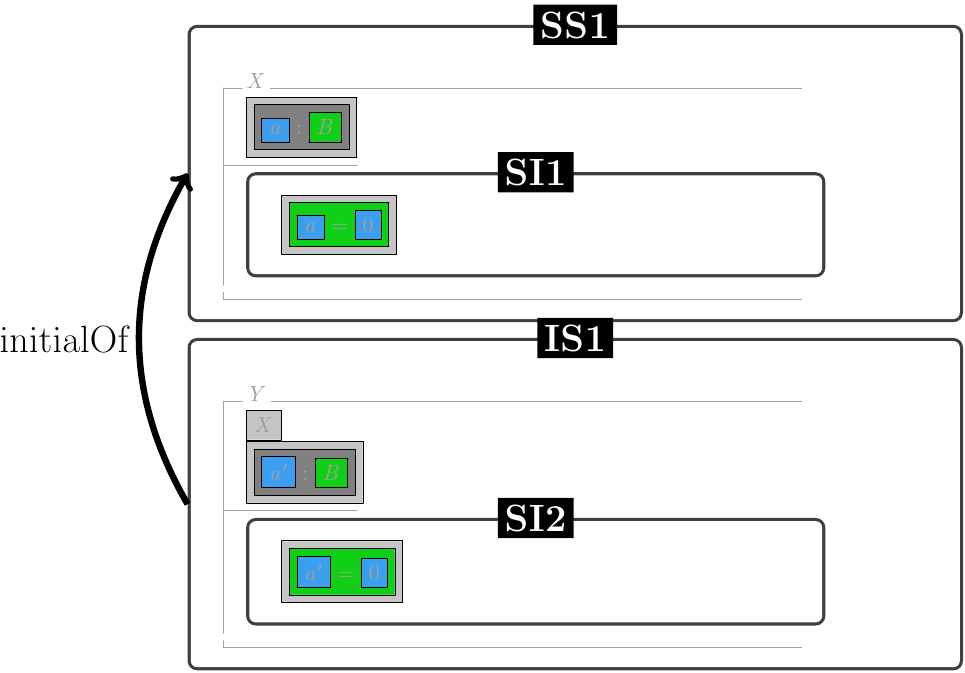
\includegraphics[scale=0.1]{Figures/Formalising/dra4.png}}
      &  
\raisebox{-\totalheight}{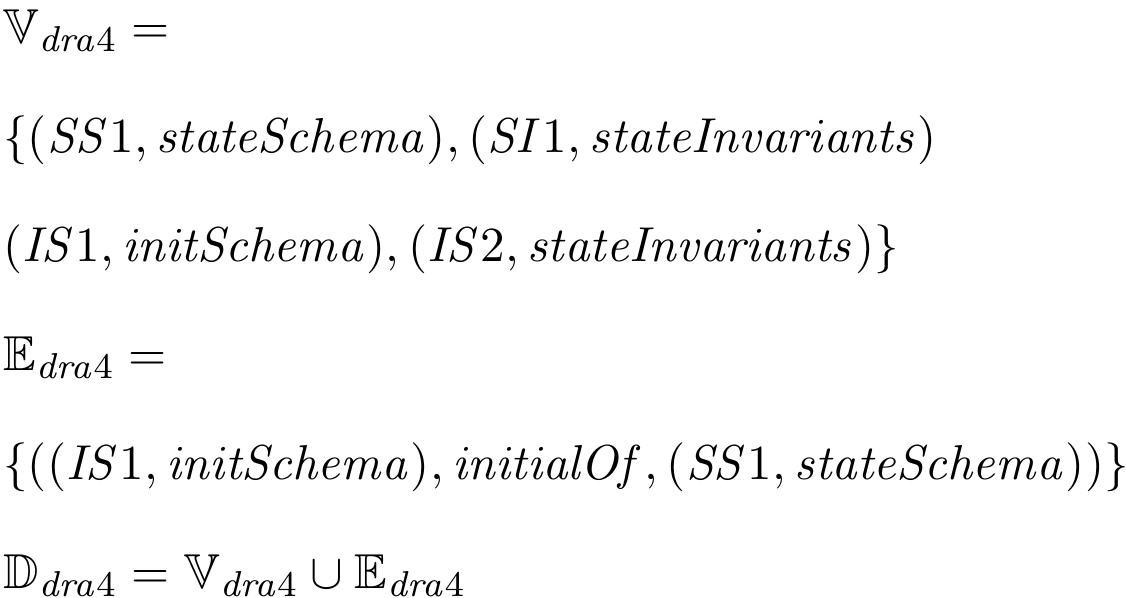
\includegraphics[scale=0.2]{Figures/Formalising/dra4txt.png}}
\\ \hline
dra5) & 
\raisebox{-\totalheight}{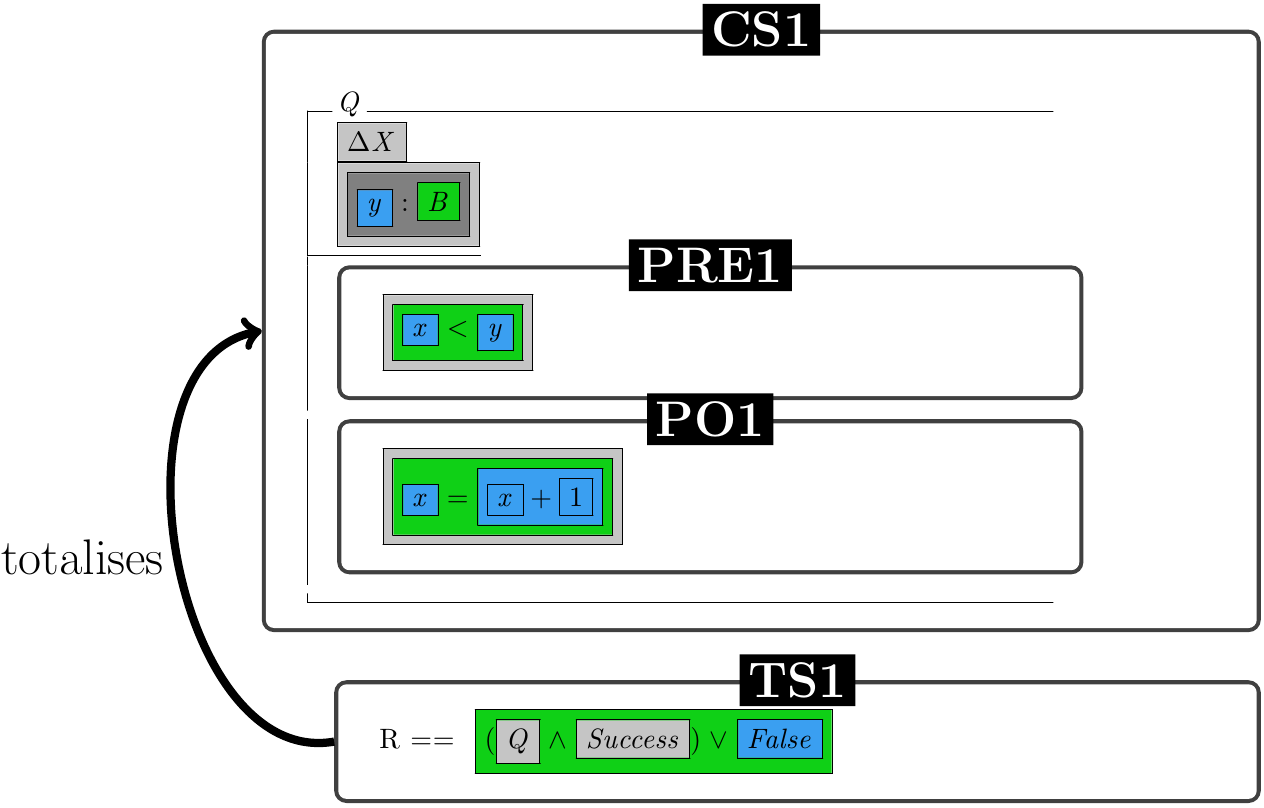
\includegraphics[scale=0.1]{Figures/Formalising/dra5.png}}
      &  
\raisebox{-\totalheight}{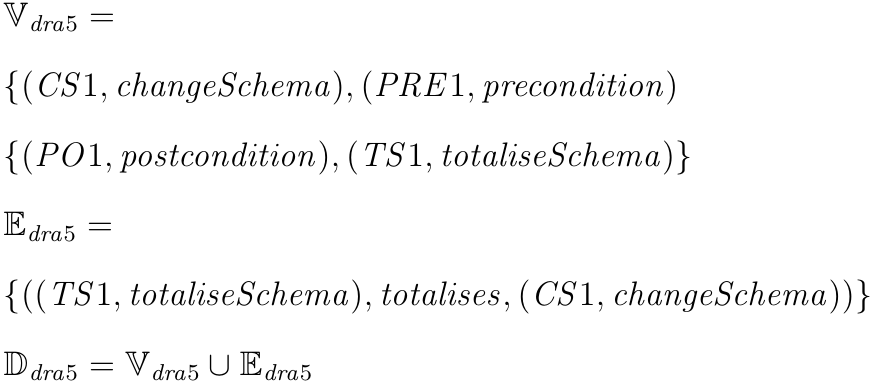
\includegraphics[scale=0.3]{Figures/Formalising/dra5txt.png}}
\\ \hline
\end{tabular}
\caption{Using the formalised definitions for vertices and edges to create a dependency graph. \label{tab:verticiesandedges}}
\end{center}
\end{table}

\begin{defin}[ChildOf] The dependency graph provides a child and parent
relationship. The definitions are as follows:

\begin{tabular}{l|l}
\hline
\textbf{Relation} & \textbf{dependency graph children}\\
\verb|\allows{A}{B}| & B childOf A \\
\verb|\requires{A}{B}| & B childOf A \\
\verb|\uses{A}{B}| & B childOf A\\
\verb|\initialOf{A}{B}| & B childOf A \\
\verb|\totalises|{A}{B}| & B childOf A \\
\hline
\end{tabular}

The goto graph also provides and child and parent relationship however some of
the relations are reversed:

\begin{tabular}{l|l}
\hline
\textbf{Relation} & \textbf{goto graph children}\\
\verb|\allows{A}{B}| & B childOf A \\
\verb|\requires{A}{B}| & B childOf A \\
\verb|\uses{A}{B}| & A childOf B\\
\verb|\initialOf{A}{B}| & A childOf B \\
\verb|\totalises|{A}{B}| & A childOf B \\
\hline
\end{tabular}

\end{defin}

Table \ref{tab:verticiesandedges} show how a dependency graph can be created
using the formal definitions for vertices and edges. The dependency graph is
directly generated from the \gls{zdra} annotated document. The relations
\emph{initialOf} and \emph{uses} are used between schemas, \emph{requires}
becomes a childOf the schema which requires it and \emph{allows} can be used
between instances within the schema (see table \ref{tab:relationsallowed}). If
the \emph{allows} relationship is used within the schema, then both the
precondition and postcondition/output becomes childrenOf the schema. Figure
\ref{fig:unnested} shows two separate schemas which are not nested within
each other, however figure \ref{fig:nested} shows the precondition PRE2 allows
the postcondition PO2 within the schema CS1, since CS1 requires PRE2 then both
PRE2 and PO2 are childrenOf CS1.

\begin{figure}[H]
\centering
\begin{minipage}{0.45\textwidth}
\centering
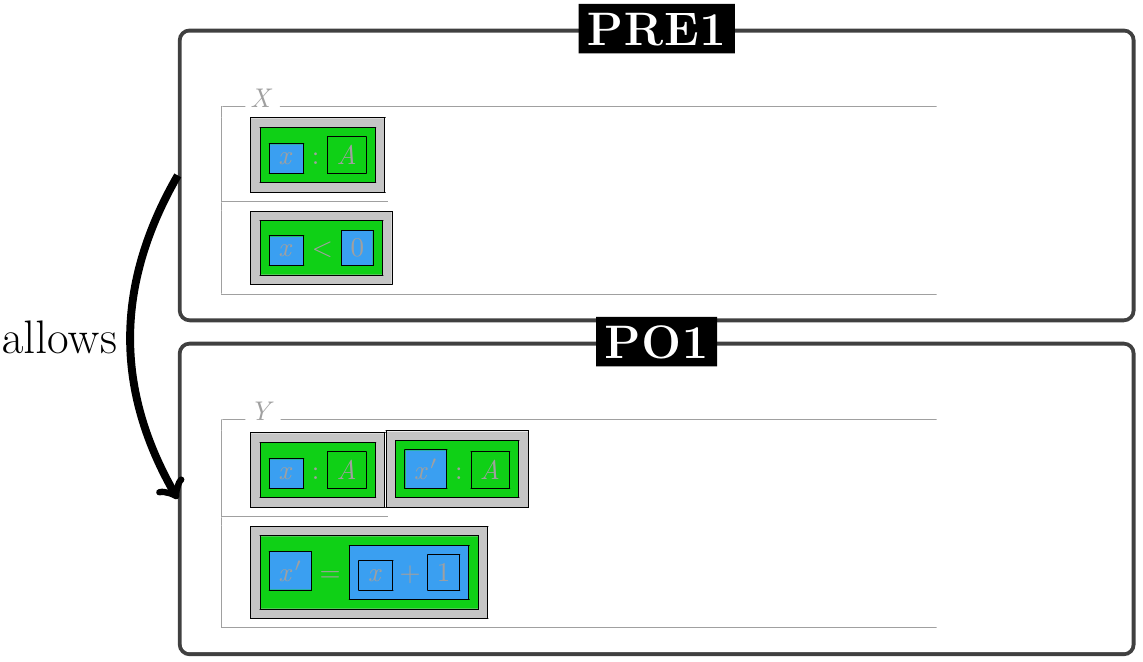
\includegraphics[scale=0.18]{Figures/Formalising/unnested.png}
\caption{Relation with un-nested precondition and postcondition.  \label{fig:unnested}}
\end{minipage}\hfill
\begin{minipage}{0.45\textwidth}
\centering
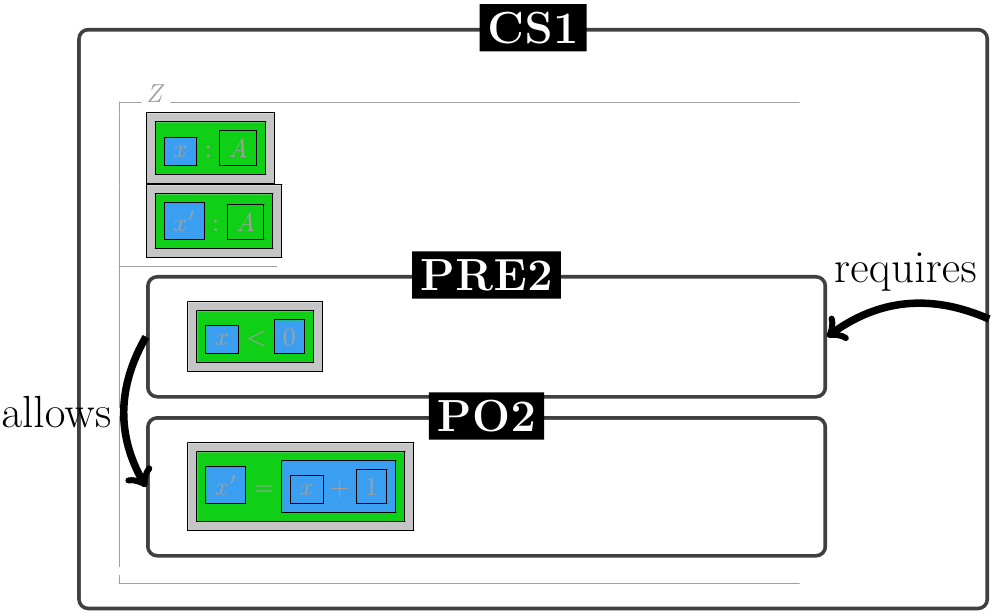
\includegraphics[scale=0.18]{Figures/Formalising/nested.png}
\caption{Relation with nested precondition and postcondition.  \label{fig:nested}}
\end{minipage}
\end{figure}

If we combine all the annotations in table \ref{tab:verticiesandedges} (whilst
adding PRE1 and PO1 in a schema named CS1) we get a fully annotated
specification and its dependency graph shown in figure \ref{fig:draspec} and
\ref{fig:draspecdep} respectively.

\begin{figure}[H]
\centering
\begin{minipage}{0.45\textwidth}
\centering
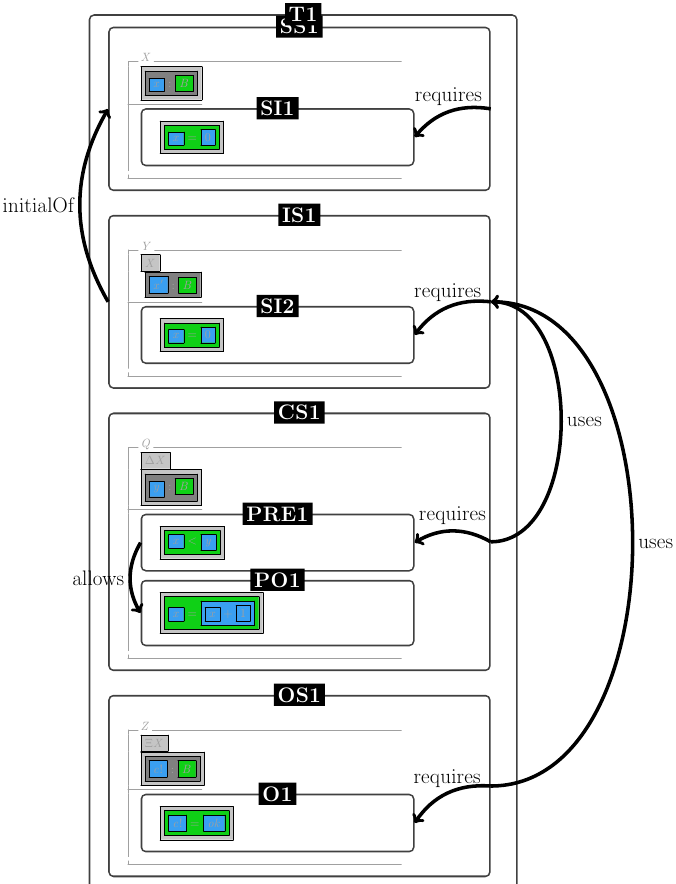
\includegraphics[scale=0.3]{Figures/Formalising/draspec.png}
\caption{All annotations from table \ref{tab:verticiesandedges} combined into one specification.  \label{fig:draspec}}
\end{minipage}\hfill
\begin{minipage}{0.45\textwidth}
\centering
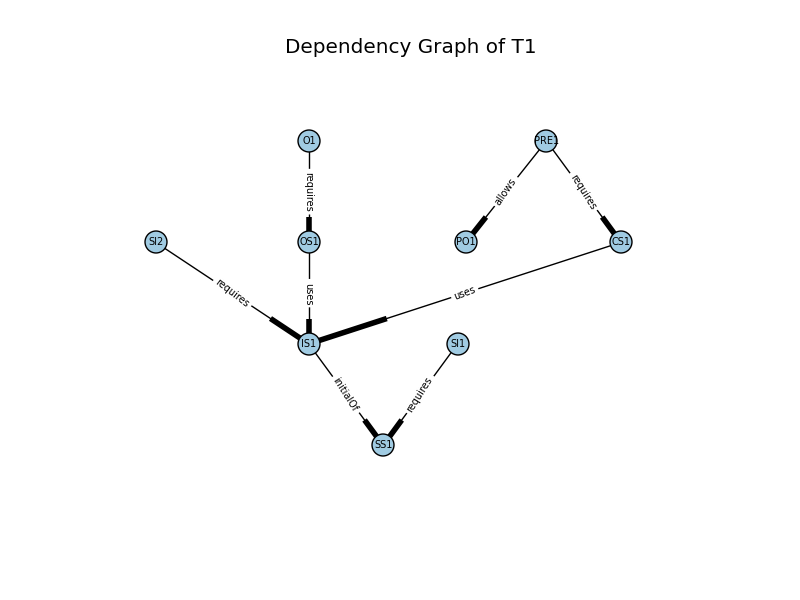
\includegraphics[scale=0.6]{Figures/Formalising/dp_text.png}
\caption{Dependency graph of the example in \ref{fig:draspec} \label{fig:draspecdep}}
\end{minipage}
\end{figure}

\noindent Since figure \ref{fig:draspec} is a combination of the annotations in
table \ref{tab:verticiesandedges} we can call this dependency graph
$\mathbb{D}_{comb}$ where \newline $\mathbb{V}_{comb} = \{ \\
(T1, theory),(SS1, stateSchema), (SI1, stateInvariants), \\ (IS1, initSchema),
(SI2, stateInvariants), (CS1, changeSchema), \\ (PRE1, precondition), (PO1,
postcondition), (OS1, outputSchema), (O1, output) \}$
\newline
\noindent and $\mathbb{E}_{comb} = \{ \\
((SS1, stateSchema), requires, (SI1, stateInvariants)) \\
((IS1, initSchema), requires, (SI2, stateInvariants)) \\
((IS1, initSchema), initialOf, (SS1, stateSchema)) \\
((CS1, changeSchema), requires, (PRE1, precondition)) \\
((PRE1, precondition), allows, (PO1, postcondition)) \\
((CS1, changeSchema), uses, (IS1, initSchema)) \\
((OS1, outputSchema), requires, (O1, output)) \\
((OS1, outputSchema), uses, (SS1, stateSchema)) \\
\}
$
\newline
\noindent and $\mathbb{D}_{comb} = \mathbb{V}_{comb} \union \mathbb{E}_{comb}$

\subsection{Generating the GoTo graph from the dependency graph}

Since the dependency graph only follows the annotations of the \gls{zdra} we
need to highlight the textual order of these annotations. For example some
annotations may be stronger then others. The order in which instances are
inputted in the theorem prover are also important so that the theorem prover may
be parsed correctly. The GoTo graph is generated using the textual order of the
dependency graph. The following definitions have been taken from
\cite{zengfirstyear}.

\begin{defin}[Textual order] We can now formalise three different kinds of
textual order when translating a dependency graph into the GoTo graph.

\begin{itemize}
\item \textbf{Strong textual order $\prec$:} This order describes an entire
entity relation between two nodes ($id_{A}$ uses $id_{B}$ would be written as
$id_{B}$ $\prec$ $id_{A}$, $id_{A}$ initialOf $id_{B}$ would be written as
$id_{B} \prec id_{A}$, $id_{A}$ totalises $id_{B}$ would be written as $id_{B}$
$\prec$ $id_{A}$).

\item \textbf{Weak textual order $\preceq$:} This order describes a sub-part
relation between two nodes ($id_{A}$ allows $id_{B}$ within a schema written as
$id_{A} \preceq id_{B}$).

\item \textbf{Common textual order $\leftrightarrow$:} This order describes a
relation between two nodes where they are both dependent on each other (Where a
draschema $id_{A}$ requires a draline of some sort $id_{B}$ is written as
$id_{A}$ $\leftrightarrow$ $id_{B}$).
\end{itemize}
\end{defin}

The dependency graph is a direct representation of the \gls{zdra} annotations
and arrows represented when compiling the \gls{zdra} annotated document. The
GoTo uses these annotations and describes the textual order of them. When
inputting a specification into an automatic theorem prover, the textual order is
important as it decides which part of the specification needs to be in-putted
first in order to parse correctly. Using the definitions from
\cite{zengfirstyear} we can now order the relations from the dependency graph.

\begin{table}[H]
\centering
\begin{tabular}{| l | l | l |}
\hline
\textbf{Relation} & \textbf{Meaning} & \textbf{Order} \\
\hline 
$id_{A}$, initialOf, $id_{B}$ & $id_{A}$ is the initial schema of $id_{B}$ &
$id_{B} \prec id_{A}$ \\
 & or $id_{A}$ initialises $id_{B}$ & \\
 \hline
$id_{A}$, uses, $id_{B}$ & $id_{B}$ is being used in $id_{A}$ & $id_{B} \prec
id_{A}$ \\
& or $id_{B}$ is needed in $id_{A}$ & \\
 \hline
 $id_{A}$, totalises, $id_{B}$ & $id_{A}$ makes the precondition in $id_{B}$
 total & $id_{B} \prec id_{A}$ \\
 \hline
$id_{A}$, allows, $id_{B}$ & $id_{A}$ is allowing $id_{B}$ to occur & $id_{A}
\preceq id_{B}$ \\
\hline
$id_{A}$, requires, $id_{B}$ & $id_{A}$ is requiring $id_{B}$ to function &
$id_{A} \leftrightarrow id_{B}$ \\
\hline
\end{tabular}
\caption{Example of ZDRa annotations and the textual order of them. \label{tab:texorder}}
\end{table}

\begin{defin}
We denote v\_1 and v\_2 to describe node 1 and node 2 respectively for example
if we have $\backslash initialof\{id_{1}\}\{id_{2}\}$ and $id_{1}$ is IS1 and
$id_{2}$ is SS1 then v\_1 would be (IS1, initialSchema) and v\_2 would be (SS1,
stateSchema).
\end{defin}

\begin{algorithm}[H] \underline{goto\_graph = directedGraph} \;
\underline{dependency\_graph = directedGraph} \; \SetAlgoLined
\uIf{$\backslash$initialof\{$id_{1}$\}\{$id_{2}$\}} 
{addEdge(v\_1, $\rightarrow$, v\_2) to dependency\_graph \; addEdge(v\_2,
$\rightarrow$, v\_1)  to goto\_graph\;}
\uIf{$\backslash$uses\{$id_{1}$\}\{$id_{2}$\}} 
{addEdge(v\_1, $\rightarrow$, v\_2) to dependency\_graph \; addEdge(v\_2,
$\rightarrow$, v\_1)  to goto\_graph \;}
\uIf{$\backslash$allows\{$id_{1}$\}\{$id_{2}$\}} 
{addEdge(v\_1, $\rightarrow$, v\_2) to dependency\_graph \; addEdge(v\_1,
$\rightarrow$, v\_2)  to goto\_graph \;}
\uIf{$\backslash$requires\{$id_{1}$\}\{$id_{2}$\}} 
{addEdge(v\_1, $\rightarrow$, v\_2) to dependency\_graph \; addEdge(v\_1,
$\rightarrow$, v\_2)  to goto\_graph \;}
\uIf{$\backslash$totalises\{$id_{1}$\}\{$id_{2}$\}} 
{addEdge(v\_1, $\rightarrow$, v\_2) to dependency\_graph \; addEdge(v\_2,
$\rightarrow$, v\_1)  to goto\_graph \;}
\caption{Algorithm to generate the dependency graph and goto. \label{alg:gotodep} }
\end{algorithm}
\vspace{0.2in}


Algorithm \ref{alg:gotodep} shows the pseudocode of the implementation on how
the dependency graph and goto graphs are created. It reads the labels created by
the user when annotating the formal specification. 

Note the edges for the relations \emph{allows} and \emph{requires} have the same
direction both in the dependency graph and the goto graph. This is because if
instance v\_1 \emph{allows} another instance v\_2 to happen then instance v\_1
must exist for instance v\_2 to exist. The relationship \emph{requires} is
between a draschema and a draline where a draschema requires a particular
draline, in the algorithm we have the dependency graph edge and goto graph edge
point in the same direction.

With the edges for relations \emph{initialof}, \emph{uses} and \emph{totalises},
algorithm \ref{alg:gotodep} changes the direction of the edges from the
dependency graph to the goto graph. If a node v\_1 is the initialOf another node
v\_2 then v\_1 initialises v\_2, therefore v\_2 must exist first for v\_1 to
initialise it. If a node v\_1 uses another node v\_2 then v\_2 must exist first
before it can be used by v\_1. This is the same with the relation
\emph{totalises}, if a node v\_1 totalises another node v\_2 then the node v\_2
must exist before the node v\_1 can totalise it.

\begin{figure}[H]
\centering
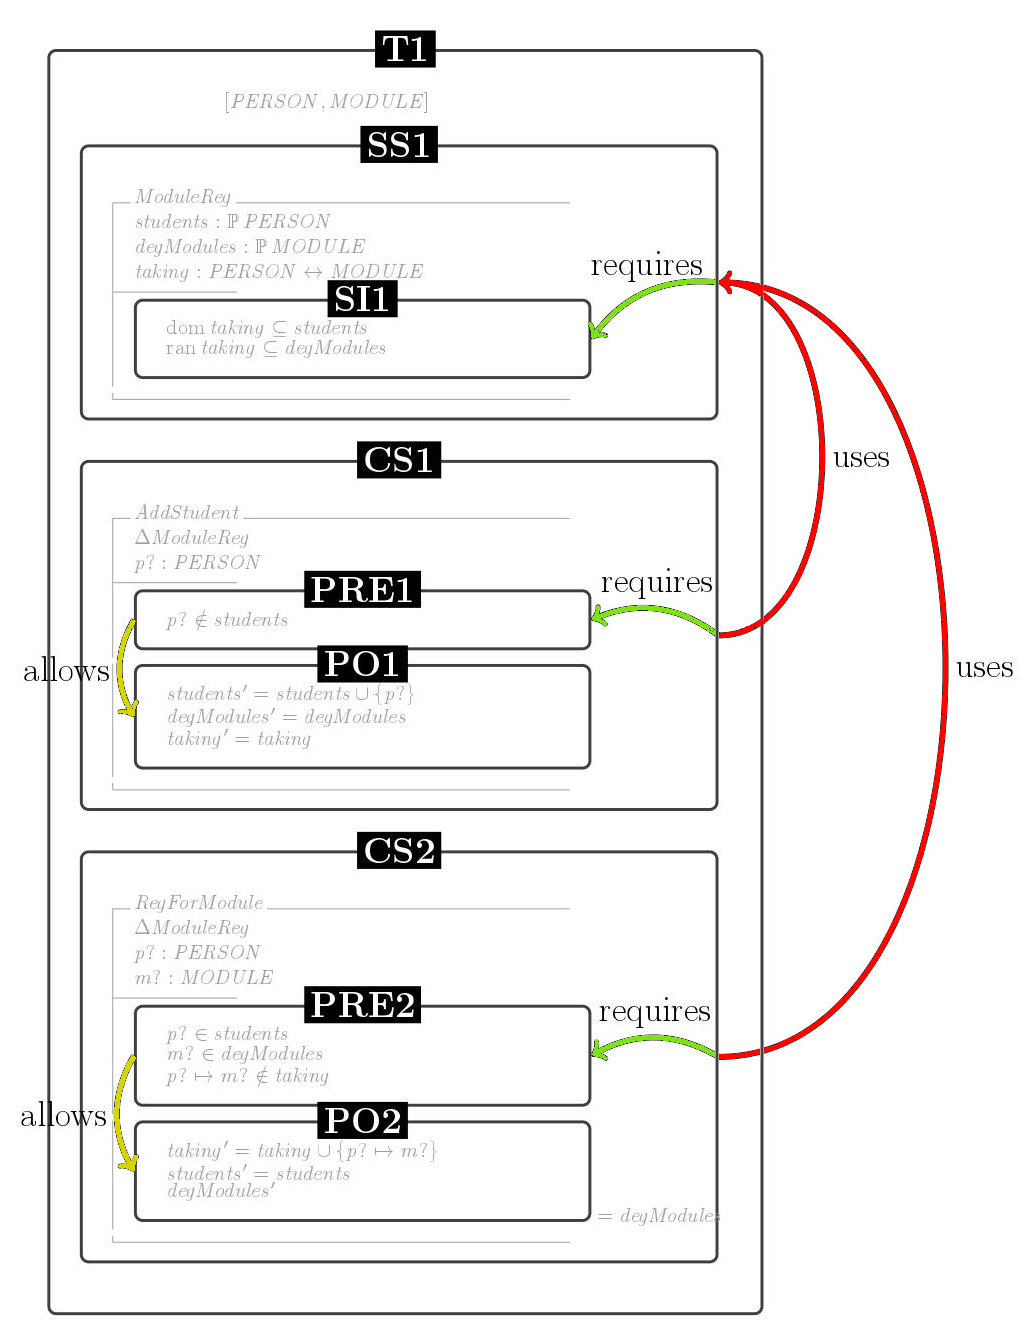
\includegraphics[scale=0.7]{Figures/Formalising/dramodule.png}
\caption{User annotated in \gls{zdra} for the modulereg specification with arrows coloured. \label{fig:zdramodule}}
\end{figure}

\begin{figure}[H]
\centering
\begin{minipage}{0.47\textwidth}
\centering
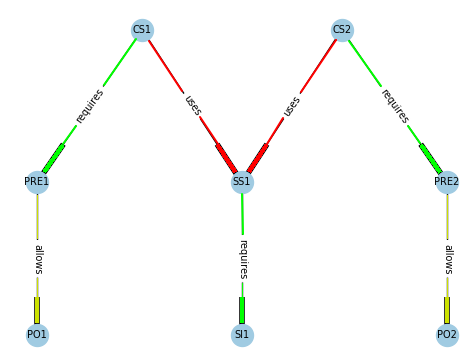
\includegraphics[scale=0.55]{Figures/Formalising/dpmodule.png}
\caption{The dependency graph of modulereg specification with arrows coloured.  \label{fig:dpmodule}}
\end{minipage}\hfill
\begin{minipage}{0.47\textwidth}
\centering
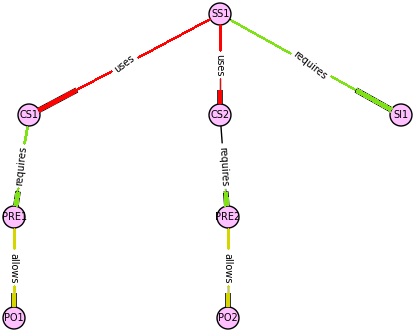
\includegraphics[scale=0.55]{Figures/Formalising/gotomodule.png}
\caption{The goto graph of modulereg specification with arrows coloured. \label{fig:gotomodule}}
\end{minipage}
\end{figure}

Figure \ref{fig:zdramodule} shows the moduleReg specification annotated in
\gls{zdra} however the colours of the arrows have been changed as to compare it
with the automatically generated dependency graph (figure \ref{fig:dpmodule})
and it's corresponding goto graph (figure \ref{fig:gotomodule}). Note the red
arrows which correspond to the `uses' relation are facing the same direction in
the user annotated document and in the dependency graph (from CS1 to SS1 and
from CS2 to SS1) however they go the opposite direction in the goto graph. This
goes the same for the green arrows which represent the `requires' relation. On
the other hand the yellow arrow, representing the `allows' relation goes in the
same direction in all three figures.

\begin{defin}[Textual order edge] We can say a textual order edge $\mathbb{O}$
is a quadruple
\begin{center}
($v_{A}, v_{B}, rel, to$)
\end{center}
where it is a relation rel, from node $v_{A}$ to node $v_{B}$ and it's textual
order to where $to \in \{\prec , \preceq , \leftrightarrow , \succ , \succeq
\}$.
\end{defin}

\begin{defin}[Graph of Textual order] A graph of textual order is a pair (V,O),
made up of a set of vertices V and a set of ordered edges O.
\end{defin}

The definitions for the `\emph{Textual order edge}' and `\emph{Graph of Textual
order}' have been taken from \cite{zengfirstyear}. The main reason for producing
a GoTo graph is to order the instances so that when printed they can parse
through an automated theorem prover. However both the dependency and goto graphs
can also be used as documents to analyse the system in question. It may also be
helpful to stakeholders in the systems project to view the system in it's
entirety and to see clearly how each component is linked with another.

\begin{table}[H]
\centering
\begin{tabular}{| c | c | c |}
\hline
\textbf{Relation} & \textbf{Textual} & \textbf{GoTo} \\
& \textbf{Order} & \textbf{Edge} \\
\hline
($v_{A}$, uses, $v_{B}$) & $v_{A} \succ v_{B}$ &
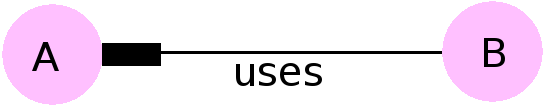
\includegraphics[scale=0.15]{Figures/Formalising/uses.png} \\
\hline
($v_{A}$, initialof, $v_{B}$) & $v_{A} \succ v_{B}$  &
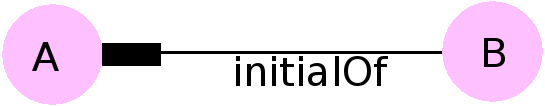
\includegraphics[scale=0.15]{Figures/Formalising/initialof.png} \\
\hline
($v_{A}$, allows, $v_{B}$) & $v_{A} \preceq v_{B}$ &
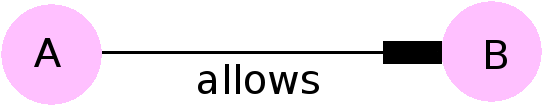
\includegraphics[scale=0.15]{Figures/Formalising/allows.png} \\
\hline
($v_{A}$, totalises, $v_{B}$) & $v_{A} \succ v_{B}$ &
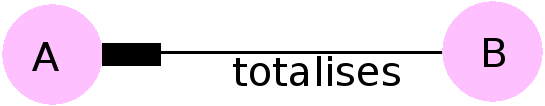
\includegraphics[scale=0.15]{Figures/Formalising/totalises.png} \\
\hline
($v_{A}$, requires, $v_{B}$) & $v_{A} \leftrightarrow v_{B}$ &
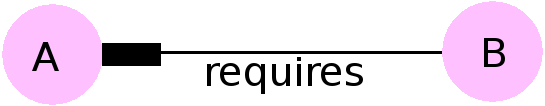
\includegraphics[scale=0.15]{Figures/Formalising/requires.png} \\
\hline
\end{tabular}
\caption{The relations represented by textual order and in the goto graph \label{tab:gotorelations}}
\end{table}

Table \ref{tab:gotorelations} shows what the textual order representation of each
relation is and how it is represented as an edge in the GoTo graph. The uses
relation has the textual order `$\succ$' where the goto graph edge would be
$(v_{A}, v_{B}, uses, \succ)$ as the relation uses would have a strong textual
order. the initialof relation is similar to the uses relation where the syntax
in the goto graph would be $(v_{A}, v_{B}, initialof, \succ)$. Totalises
relation also has a similar edge to uses and initialof as the syntax for the
goto graph edge would be: $(v_{A}, v_{B}, totalises, \succ)$. The allows
relation has a weak textual order where the goto edge syntax would be $(v_{A},
v_{B}, allows, \preceq)$. The requires relation uses the textual symbol
`$\leftrightarrow$' as the requires describes a relation that is $subpart\ of$,
for example if we have $v_{A}$, requires, $v_{B}$ then this describes a relation
that $v_{A}$ is $subpart\ of$ $v_{B}$ therefore the goto edge syntax would be
$(v_{A}, v_{B}, requires, \leftrightarrow)$.

\begin{figure}[H]
\centering
\begin{minipage}{0.45\textwidth}
\centering
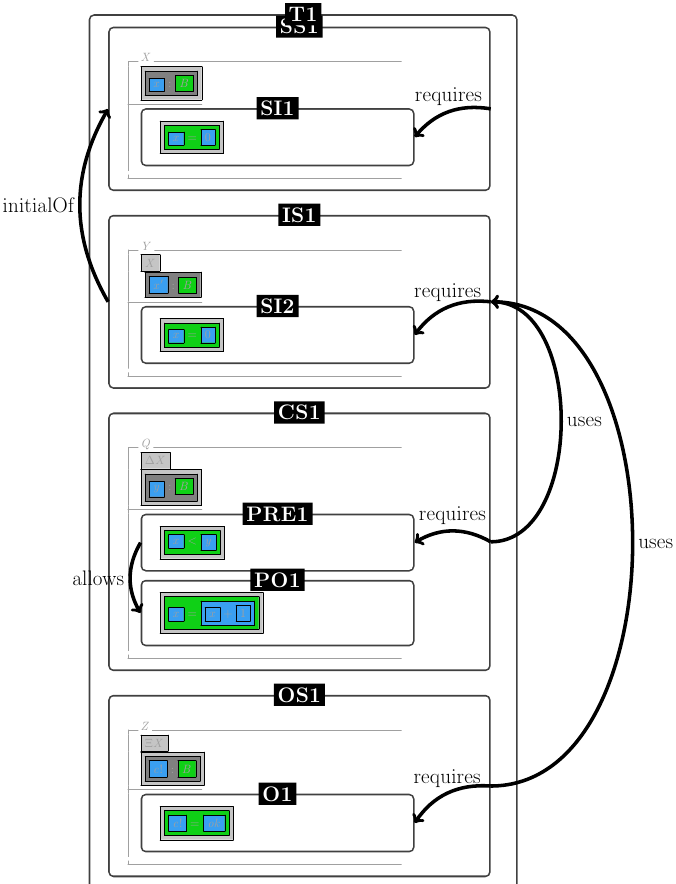
\includegraphics[scale=0.3]{Figures/Formalising/draspec.png}
\caption{All annotations from table \ref{tab:verticiesandedges} combined into one specification.  \label{fig:draspeca}}
\end{minipage}\hfill
\begin{minipage}{0.45\textwidth}
\centering
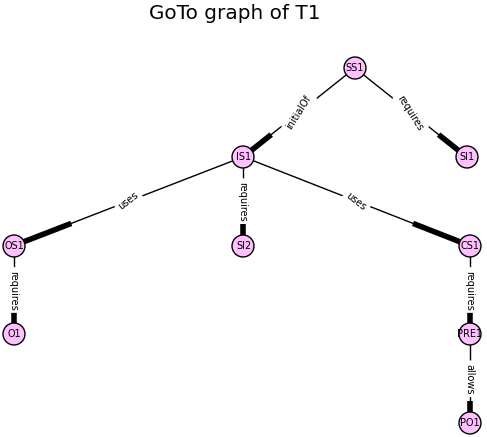
\includegraphics[scale=0.6]{Figures/Formalising/goto_text.png}
\caption{Goto graph of the example in \ref{fig:draspeca} \label{fig:gotospecdep}}
\end{minipage}
\end{figure}

Therefore our nodes would be:

$\mathbb{V}_{figure\ \ref{fig:gotospecdep}}= \{ \\
(T1, theory),(SS1, stateSchema), (SI1, stateInvariants), \\ (IS1, initSchema),
(SI2, stateInvariants), (CS1, changeSchema), \\ (PRE1, precondition), (PO1,
postcondition), (OS1, outputSchema), (O1, output) \}$\\

\noindent and our edges would be: \\
$\mathbb{O}_{figure\ \ref{fig:gotospecdep}}= \{ \\
((SS1, stateSchema), (SI1, stateInvariants), requires, \leftrightarrow) \\
((IS1, initSchema), (SI2, stateInvariants), requires, \leftrightarrow) \\
((IS1, initSchema),  (SS1, stateSchema), initialOf, \succ) \\
((CS1, changeSchema), (PRE1, precondition), requires, \leftrightarrow) \\
((PRE1, precondition), allows, (PO1, postcondition), allows, \preceq) \\
((CS1, changeSchema), (IS1, initSchema), uses, \succ) \\
((OS1, outputSchema), (O1, output), requires, \leftrightarrow) \\
((OS1, outputSchema), (SS1, stateSchema), uses, \succ) \\
\} $\\

Therefore the goto graph would be the pair $\mathbb{V}_{figure\
\ref{fig:gotospecdep}}, \mathbb{O}_{figure\ \ref{fig:gotospecdep}}$ which we
could use to input into a theorem prover.

\section{What is a General Proof Sketch}
\label{sec:zdra2gen}

When checking for ZDRa correctness the program adds all the annotated chunks
into a dependency graph and a GoTo graph. Both these graphs are directed graphs.

We then run an algorithm on the GoTo graph to generate a proof skeleton.
Algorithm \ref{alg:code} shows part of the code in generating this proof sketch.

%\begin{figure}[H] 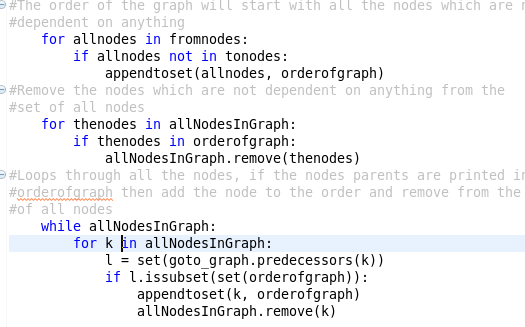
\includegraphics[scale=0.5]{Figures/skeleton/code.png}
%\caption{Part of the algorithm to create a proof sketch.} \label{fig:code}
%\end{figure}


\begin{algorithm}[H] \KwData{instances are known as `nodes'}
\KwData{OrderOfGraph is an ordered graph which lists the general proof skeleton}
\KwData{ListOfAllNodes is an unordered list containing all nodes} \BlankLine
\For{each node in ListOfAllNodes}{
\eIf{node is a root}
{push to OrderOfGraph} {$nothing$}} \For{each node in ListOfAllNodes}{\eIf{node
in OrderOfGraph}{remove node from ListOfAllNodes}{$nothing$}} \While{there are
nodes in ListOfAllNodes}{\For{each node in ListOfAllNodes}{predes = predecessor
of each node\; \eIf{predes is a subset of OrderOfGraph}{push each node to
OrderOfGraph\; remove each node\;}{$nothing$}}}
\caption{Part of the algorithm to create a proof sketch\label{alg:code}.}
\end{algorithm}

\section{Creating the Graph}

Here we show how a Proof skeleton is calculated using the Goto graph created
when running the ZDRa check on a specification.

\begin{figure}[H]
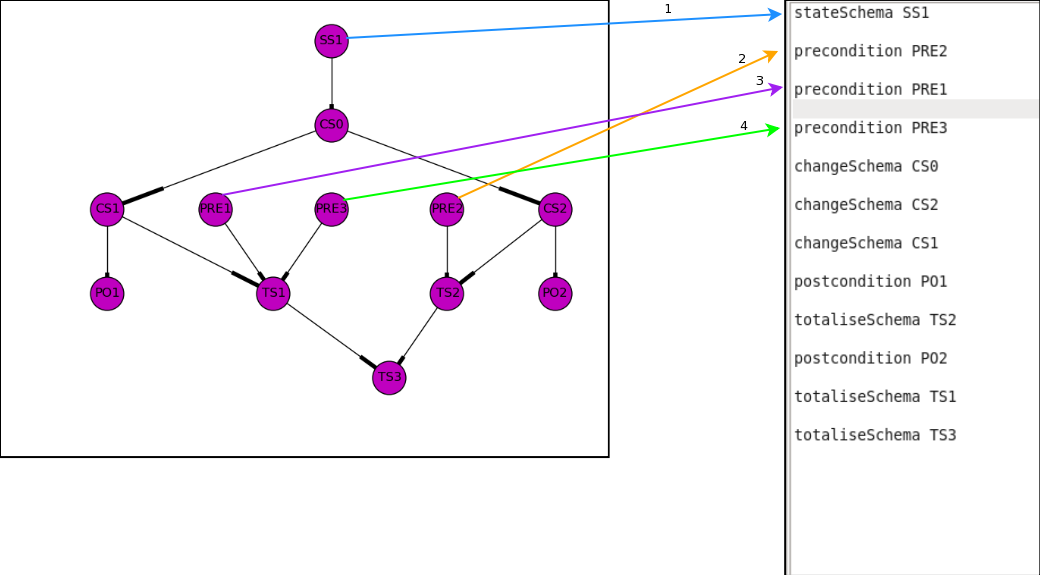
\includegraphics[scale=0.3]{Figures/skeleton/1.png}
\caption{GoTo graph and proof skeleton of vending machine step 1.}
\label{fig:1}
\end{figure}

First of all the program looks at all the nodes of the GoTo graph and prints out
all the nodes which are not dependent on anything. That is, they may have
successors but they have no predecessors, they do not use or need anything else
and can stand by themselves. These nodes can be printed in any order, so in
diagram \ref{fig:1} we see that we have SS1, PRE1 PRE2 and PRE3 all printed.

\begin{figure}[H]
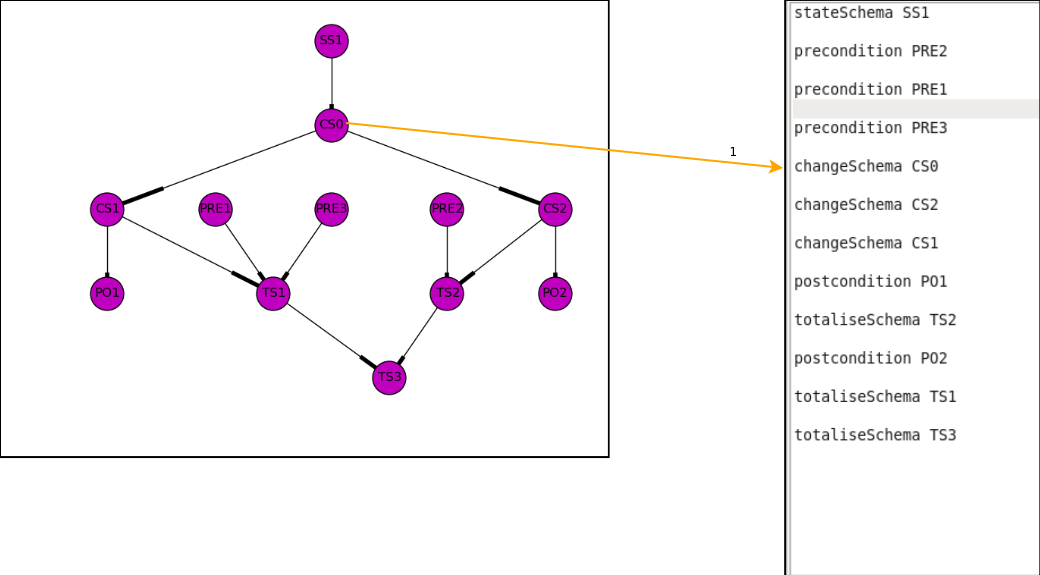
\includegraphics[scale=0.3]{Figures/skeleton/2.png}
\caption{GoTo graph and proof skeleton of vending machine step 2.}
\label{fig:2}
\end{figure}

The next part of the algorithm checks whether there exists a node in the GoTo
graph where all of its parents are printed out in the proof skeleton. Figure
\ref{fig:2} shows that the next node to be in the proof skeleton is CS0. 

\begin{figure}[H]
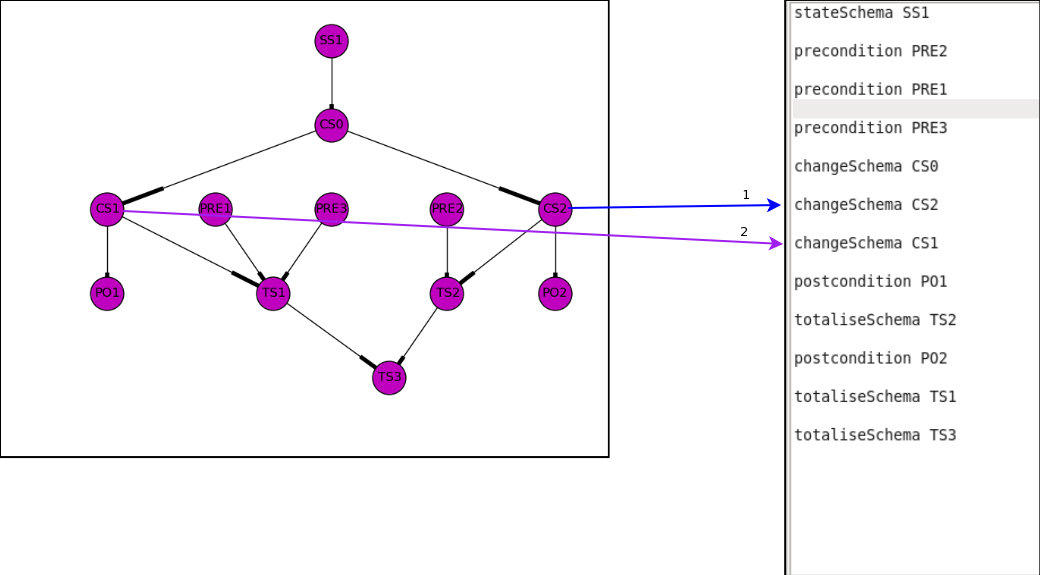
\includegraphics[scale=0.3]{Figures/skeleton/3.png}
\caption{GoTo graph and proof skeleton of vending machine step 3.}
\label{fig:3}
\end{figure}

The next part we see that after CS0 is added to the proof skeleton then both
CS1, and CS2 can be added. This is shown in figure \ref{fig:3}.

\begin{figure}[H]
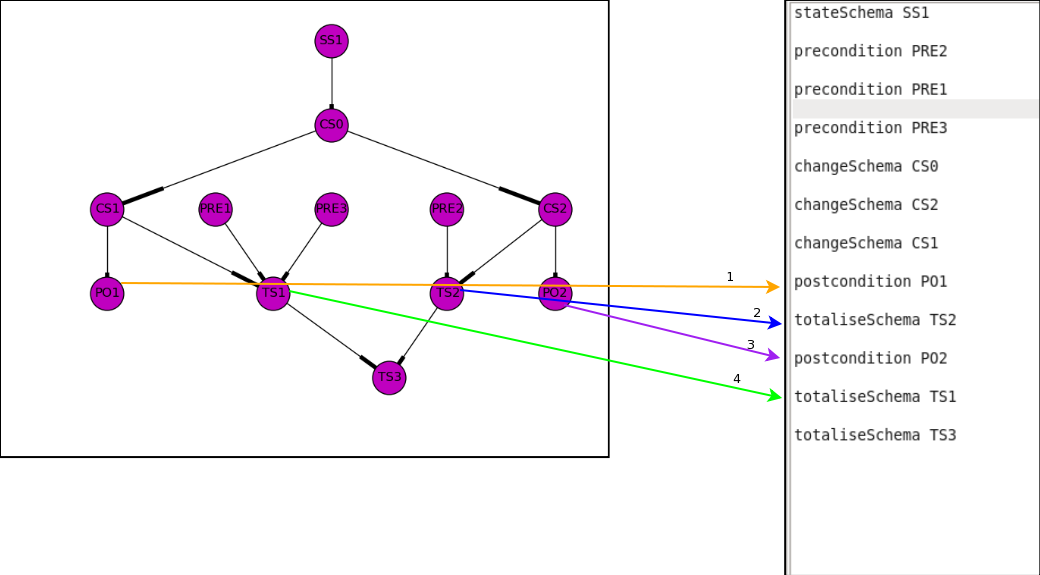
\includegraphics[scale=0.3]{Figures/skeleton/4.png}
\caption{GoTo graph and proof skeleton of vending machine step 4.}
\label{fig:4}
\end{figure}

Figure \ref{fig:4} shows the next stage of adding nodes to the Proof Skeleton.
Since CS1 and CS2 are now added to the proof skeleton then the next row of nodes
can be added. Since PO1 only had one parent (CS1) it is added first, PO2 also
had one parent (CS2) it is added second. The others had more parents which are
already in the proof sketch so they are added next randomly.

\begin{figure}[H]
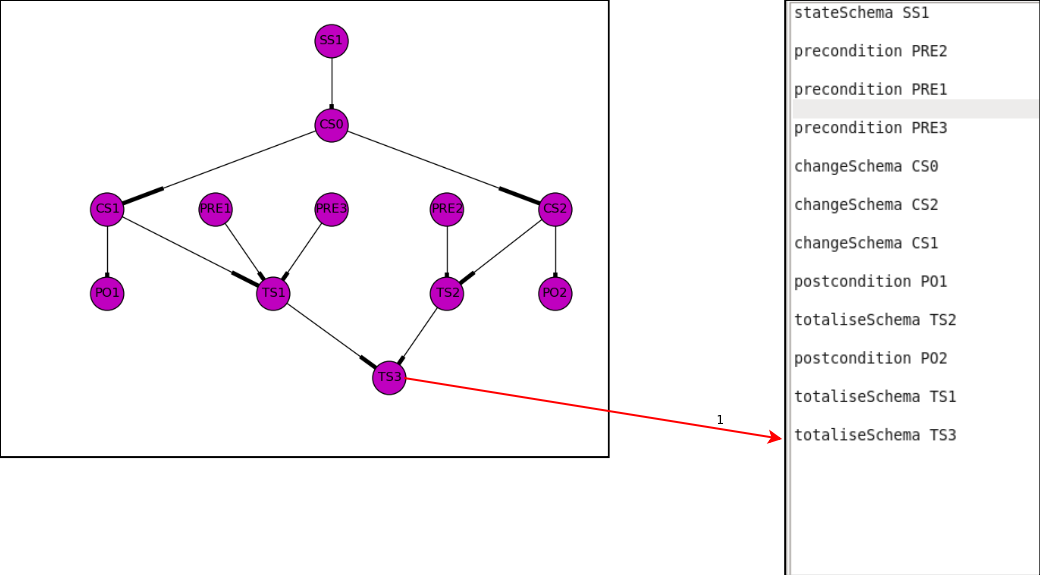
\includegraphics[scale=0.3]{Figures/skeleton/5.png}
\caption{GoTo graph and proof skeleton of vending machine step 5.}
\label{fig:5}
\end{figure}

We come to the final stage of the dependency graph, when all the nodes are in
the dependency graph except for one which is added to the end.

\section{Proof Obligations}
\label{sec:proofobl}

There are many properties one may wish to prove about their specification. These
certain properties are called proof obligations. Proof obligations for formal
notations are an entire research area in their own right. However as the
\gls{zmath} framework concentrates on giving the novice an idea of how to prove
their specification we will focus on checking the specification for consistency.
Using the description in \cite{DBLP:conf/icsea/WenMZ06}, checking the
specification is consistent can fall under two categories:

\begin{itemize}
\item POb1, Feasibility of an operation
\item POb2, Other specific proof obligation for the chosen specification
\end{itemize}

We use the syntax \textit{Context} $\vdash$ \textit{predicate} taken from
\cite{DBLP:conf/icsea/WenMZ06} to define the proof obligations.

\subsection{POb1, Proof Obligation type 1}
\label{subsec:pob1}

\begin{defin}\label{defa}POb1\\

$Context \vdash \exists (var::type)* \bullet PRE\# \land PO\# \longrightarrow
SI\# \land SI\#'$\\

\noindent where $(var::type)*$ are the variables and z-types used in the schema
with their types. We denote $*$ to declare there is 1 or many variables and
types. $SI\#$ is the state Invariants of the specification, $SI\#'$ is the state
invariants prime in the specification, $PRE\#$ is the precondition of the
schema, $PO\#$ is the post operation of the schema and $\#$ is some arbitrary
number which the user has labeled their instance with.
\end{defin}

POb1 shows the feasibility of an operation. When an operation can transfer a
state to another state in the state space (a $\Delta$ schema). If an operation
is feasible, the preconditional state and postconditional state should satisfy
the state invariants of the specification.

Again by using the ModuleReg specification we can see a proof obligation is
needed when adding a student doesn't change the state invariants of the
specification.

\begin{verbatim}
lemma AddStudentDoesntChangeSI:
"(\<exists> taking taking'  :: (PERSON * MODULE) set.
 \<exists> degModules degModules':: MODULE set.
 \<exists> students students':: PERSON set.
  \<exists> p :: PERSON.
(students' = students \<union> {(p)}) 
\<and> (taking' = taking)
\<and> (degModules' = degModules)
\<longrightarrow> ((Domain taking \<subseteq> students)
\<and> (Range taking \<subseteq> degModules)
\<and> (Domain taking' \<subseteq> students')
\<and> (Range taking' \<subseteq> degModules'))) "
\end{verbatim}

The ZDRa syntax of this proof obligation would be :

\begin{verbatim}
lemma AddStudentDoesntChangeSI:
" \<exists> (*CS1_variables :: CS1_TYPES*).
(PRE1)
\<and> (PO1)
\<longrightarrow> ((SI1)
\<and (SI1'))"
\end{verbatim}

 The ZDRa syntax of the proof obligation stays that there exists some variables
 of the operational schema where the precondition (PRE1) \emph{and}
 postCondition (PO1) imply that the stateInvariants (SI1) and stateInvariants
 prime hold.

\subsection{POb2, Proof Obligation type 2}

As POb2 are any other relevant properties users wish to prove about the
specification we can not formally define it. However an example would be if
there existed a specification where an operator which added a member to a club
and then removed a member from the club. Then the amount of members should be
the same after both operators have completed the task.

One such example is in the ModuleReg specification the RegForModule schema
postcondition shows that \verb|(taking' = taking ∪ {(p, m)}) | therefore if this
were to happen then we should make sure that \verb|taking'| is not empty after
the operation. This proof obligation is very specific to the ModuleReg
specification and the user would need to write and check this themselves. To do
such we have the following lemma:

\begin{verbatim}
lemma notEmpty:
"(taking' = taking \<union> {(p,m)}) 
\<longrightarrow> (taking' \<noteq> {})"
\end{verbatim}

Where the name of the lemma is \verb|notEmpty| then the postOperation of the
ChangeSchema is \verb|(taking' = taking \<union> {(p,m)}) | then checking that
the set is not empty follows the right arrow \verb|(taking' \<noteq> {})|.

POb1 can be automate. Since POb2 is specification specific, each user will need
to define these themselves if they so wish.

\subsection{Proof Obligations in the General Proof Skeleton}

Since the POb2 are specific to the specification only POb1 are automatically
added. They are generated as `\emph{lemma's}' in the general proof skeleton. 

%\begin{algorithm}[H] \KwData{instances are known as `nodes'}
%\KwData{OrderOfGraph is an ordered graph which lists the general proof
%skeleton} \KwData{ListOfAllNodes is an unordered list containing all nodes}
%\For{dupa}{If node is a root\; push to OrderOfGraph\;} \For{each node in
%ListOfAllNodes}{if node in OrderOfGraph\; remove node from ListOfAllNodes\;}
%\While{there are nodes in ListOfAllNodes}{\For{each node in
%ListOfAllNodes}{predes = predecessor of each node\; if predes is a subset of
%OrderOfGraph\; push each node to OrderOfGraph\; remove each node\;}
%}
%\caption{Part of the algorithm to create a proof sketch\label{fig:code}.}
%\end{algorithm}

%\begin{figure}[H] 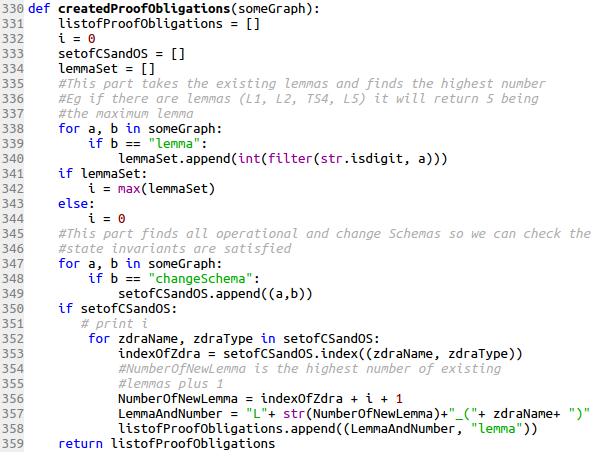
\includegraphics[scale=0.6]{Figures/skeleton/pobcode.png}
%\caption{Part of the algorithm to create Proof Obligation ZDRa names.}
%\label{fig:codepob} \end{figure}

\begin{algorithm}[h] \KwData{listOfProofObligations is a set containing the ZDRa
names of properties to prove} \KwData{i is the highest value of lemma, e.g if we
have the following lemmas \[L1, L2, L3\]} \KwData{setOfCS is a set containing
all the ZDRa names which are a change schema} \KwData{lemmaset is a set
containing all ZDRa names of existing lemmas} \BlankLine \For{(ZDRa name,
instance type) in GoTo graph}{Add ZDRa name to lemmaSet}
\eIf{there are elements in lemmaSet}{i becomes highest value lemma}{i = 0}
\For{(zdra Name, instance type) in GoTo graph}{
\eIf{instance type is a changeSchema}{add zdra Name to setOfCS}{$nothing$}
} \eIf{there are elements in setOfCS}{\For{(zdra name, instance type) in
setOfCS}{indexOfElement = index of (zdra name, instance type)\; numberOfNewLemma
= i + indexOfElement + 1\; ZDRaNameOfNewLemma = `L' + numberOfNewLemma\; push
(ZDRaNameOfNewLemma, "lemma") to general proof skeleton\;}}{$nothing$}
\caption{Part of the algorithm to create Proof Obligation ZDRa names \label{alg:codepob}.}
\end{algorithm}

The proof obligations which check that changeSchema's and outputSchema's follow
the stateInvariants are added to the original general proof skeleton. The
general proof skeleton starts of with being an ordered list (GPSaOL), then the
algorithm for generating a list of proof obligations is run and added to the
original proof skeleton. Algorithm \ref{alg:codepob} shows the algorithm which
creates the ordered list of proof obligations.

Lines 338-344 find all the existing lemma's in the \gls{gpsol} and sets \emph{i}
to be the highest number. For example if there are existing lemmas in
\gls{gpsol} (L1, L2, L3), then \emph{i} becomes 3. If there are no existing
lemmas in \gls{gpsol} then \emph{i} stays as 0. Lines 347-250 take all the
elements which are \emph{changeSchema} instances and adds them to a list of
\emph{setCSandOS}. Then lines 350-359 loops through all the changeSchema's,
takes the \gls{zdra} name, adds L + a number + \gls{zdra} name and adds it to
the \emph{listOfProofObligations}.

\paragraph{For Example}

if we had the following \gls{gpsol}: \\
\noindent [(SS1, stateSchema), (IS1, initialSchema), (CS1, changeSchema), (CS2,
changeSchema), (TS1, totaliseSchema)] \\
Then in this case:
\begin{itemize}
\item lemmaSet = []
\item i = 0
\item setofCsandOs = [(CS1, changeSchema), (CS2, changeSchema)]
\end{itemize}

Then for each element in setofCsandOs we would add the new elements (L1\_CS1,
lemma) and (L2\_CS2, lemma) to the ordered list \emph{listOfProofObligations}.

The new \gls{gpsol} would then become [(SS1, stateSchema), (IS1, initialSchema),
(CS1, changeSchema), (CS2, changeSchema), (TS1, totaliseSchema), (L1\_CS1,
lemma) and (L2\_CS2, lemma)]

If for example the original \gls{gpsol} was \\
\noindent [(SS1, stateSchema), (IS1, initialSchema), (CS1, changeSchema), (CS2,
changeSchema), (TS1, totaliseSchema), (L1, lemma), (L2, lemma)]\\
Then then new proof obligation lemmas would be (L3\_CS1, lemma) and (L4\_CS2,
lemma) as we would already have L1 and L2.

\begin{figure}[H]
\centering
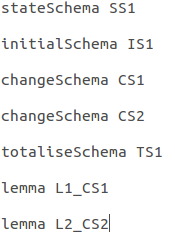
\includegraphics[scale=0.5]{Figures/skeleton/proofskeletonwithpo.png}
\caption{Example of a General Proof Skeleton with lemma's.}
\label{fig:gpswithpo}
\end{figure}

An example of a General Proof Skeleton with added proof obligations is shown in
Figure \ref{fig:gpswithpo}. The changeSchema's in this specification are CS1 and
CS2. Therefore to make sure the changeSchemas do not change the state of the
specification and comply with the state invariants the two lemma's L1\_CS1 and
L2\_CS2 have been added.

\subsubsection{Proof Obligations in specification examples}
Since the vending machine specification (appendix \ref{app:vm2}) doesn't have
any stateInvariants then the \gls{gps} will not have any added proof
obligations to check for consistence. That is we can't check that the
postconditions do not change the state if the state has no restrictions. However
the birthdaybook example (appendix \ref{app:bb3}) does have stateInvariants.
Therefore we must add properties to check that any changeSchema's follow the
state restrictions. Part of the birthdaybook \gls{gps} is shown in figure
\ref{fig:bbgps}. Since there are stateInvariants (SI1) and a changing state
Schema (CS1) then the proof obligation \texttt{L1\_(CS1)} has been added to the
\gls{gps}.

\begin{figure}[H]
\begin{verbatim}
stateSchema SS1 
stateInvariants SI1 
initialSchema IS1 
postcondition PO2 
outputSchema OS1 
precondition PRE2 
changeSchema CS1 
totaliseSchema TS1 
.......
lemma L1_(CS1) 
\end{verbatim}
\caption{Part of the GPSa for the birthdayBook example. (Full version shown in appendix \ref{app:bb3}) \label{fig:bbgps}}
\end{figure}

\section{Conclusion}
\label{sec:skeletonsConclusion}

This chapter describes how the \gls{zdra} program uses the GoTo graph to
generate a general proof skeleton (step 2$\rightarrow$3 in figure
\ref{fig:steps}). The general proof skeleton is an automatically generated .txt
file which displays the order in which this instances must go in a theorem
prover to be logically correct. This chapter gives a basic understanding of
proof obligations for Z and examples which proof obligations are automatically
generated when translating Z specifications into Isabelle. We give a formal
definition of the proof obligation to check for consistency of the state
invariants and show an example. The next chapter describes how the general proof
skeleton is translated into Isabelle syntax.
